\chapter{Konstrukcja mechaniczna urządzenia}
\label{cha:constr}
W~tym rozdziale, po wybraniu rodzaju konstrukcji oraz platformy sprzętowej, autor przedstawia zastosowane komponenty oraz generalną konstrukcję mechaniczną projektu.
\section{Zastosowane komponenty}
\label{sec:komponenty}
Aby skonstruować kompletny system pasywno-aktywnego tłumienia hałasu, autor zbudował swój projekt na bazie prostych, komercyjnych nauszników tłumiących, stosowanych w~budownictwie lub przemyśle. Nauszniki te stanowią część tłumiącą pasywnie. Do stworzenia i~zaimplementowania części aktywnej układu zastosowano wymienione poniżej elementy analogowe oraz cyfrowe, przy czym elementy cyfrowe są wymienione każdy z~osobna, pomimo bycia integralną częścią mikrokontrolera.
\begin{enumerate}
	\item Analogowe:
	\begin{itemize}
		\item 2x Pojemnościowy mikrofon elektretowy CMA-4544PF-W\\
		Jeden główny (feedforward) oraz jeden odsłuchowy (feedback) wewnątrz muszli.
		\item 2x Przedwzmacniacz mikrofonowy Adafruit MAX4466\\
		Wzmacniacz operacyjny zoptymalizowany przez producenta pod kątem wykorzystania z~mikrofonami. Autor zakupił przedwzmacniacz połączony przez producenta z~wyżej wymienionym mikrofonem w~ramach jednej płytki. Należy pamiętać o~potrzebie wprowadzenia korekty fazy po przesunięciu jej przez ten komponent. Producent deklaruje 
		\item Wzmacniacz audio klasy D Adafruit PAM8302\\
		Ten wzmacniacz mono o~mocy \SI{2.5}{\W} skonstruowany jest do współpracy z~głośnikami o~impedancji od \SI{4}{} do \SI{8}{\ohm}. Producent deklaruje sprawność w~zakresie 85-88\% \cite{speakeropamp} oraz niskie przesterowania (10\% THD+N).
		
		\item Głośnik MG15 \SI{0.1}{\W}; \SI{8}{\ohm}
	\end{itemize}
	\item Cyfrowe:
	\begin{itemize}
		\item 2x Przetwornik analogowo-cyfrowy\\
		Autor zdecydował się użyć dwóch osobnych przetworników do akwizycji sygnału z~mikrofonów, aby uniknąć przesterowań i~przesłuchów, które inaczej byłyby bardzo silnie wdrożone do toru pomiarowego w~przypadku użycia jednego przetwornika. Wiąże się to z~dużą podatnością na szum, którą charakteryzuje się rozdzielający kanały multiplekser większości przetworników A/C. Zmniejsza to też nieznacznie opóźnienia w~przetworzeniu sygnału, gdyż można wtedy skonfigurować przetworniki w~trybie mierzenia pojedynczego kanału, a~nie skanowania po kolei wszystkich dostępnych~16. Przetwornik realizuje algorytm SAR\footnote{Sukcesywna Aproksymacja (ang. Successive Approximation Register, inaczej próbkowanie bitowe)}.\\
		Warto zauważyć, że przetworniki dostępne na płytce użytej przez autora mają rozdzielczość 12-bit, co pozostawia pewne pole do poprawy projektu i~wyboru komponentów, ale jednocześnie zapewnia wystarczający poziom dokładności.
		\item 2x Kontroler DMA\footnote{Bezpośredni Dostęp do Pamięci (ang. Direct Memory Access)}\\
		Jeden z~kontrolerów użyty jest do transferu danych z~przetworników~A/D do pamięci mikrokontrolera STM32, zaś drugi do transferu po przeprowadzeniu obliczeń z~pamięci do przetwornika D/A. Transfer w~pierwszym przypadku dokonywany jest w~trybie ciągłym, a~więc po każdym przerwaniu do DMA zgłoszonym przez przetwornik na końcu konwersji. W~drugim przypadku, transfer wywoływany jest po każdym skończonym cyklu obliczeniowym.
		\item NVIC (Nested Vectored Interrupt Controller)\\
		Kontroler przerwań (zagnieżdżonych), który przyspiesza ich obsługę.
		\item Mikroprocesor\\
		Główna jednostka obliczeniowa.
		\item FPU (Floating Point Unit)
		Jednostka dedykowana do obliczeń zmiennoprzecinkowych 32-bit (a~więc typu float). Znacznie przyspiesza obliczenia na ułamkach, należy jednak pamiętać, że nie działa dla typu double (więc 64-bit). 
		\item Przetwornik cyfrowo-analogowy\\
		Do celu prototypowego użyto jednego kanału wyjściowego, aby przetestować działanie systemu w~jednolitej, odgrodzonej przestrzeni sferycznej. Konwersja sygnału na postać analogową następuje automatycznie, bez wywołania, przy każdej wykrytej zmianie słowa bitowego podanego na rejestr prowadzący do przetwornika DAC.
	\end{itemize}
\end{enumerate}

\section{Schemat i konfiguracja układu}
\label{sec:config}
Uproszczony schemat w~wersji graficznej został przedstawiony przez autora na rysunku \ref{fig:schemat1}. Podstawową zasadą działania systemu jest:
\begin{enumerate}
	\item Akwizycja sygnału przez mikrofon główny oraz odsłuchowy.
	\item Wzmocnienie sygnału przez przedwzmacniacz mikrofonowy.
	\item Konwersja analogowego sygnału do postaci cyfrowej w~przetworniku ADC.
	\item Transfer danych przez kontroler DMA do pamięci urządzenia.
	\item Odczyt danych z~mikrofonu głównego z~pamięci i~przetworzenie ich w~filtrze FIR.\\
	Odczyt danych z~mikrofonu odsłuchowego i~przetworzenie ich w~module strojenia LMS.
	\item Jednoczesne przekazanie danych z~mikrofonu głównego do modułu strojenia filtra LMS.
	\item Przestrojenie filtra na podstawie algorytmu LMS.
	\item Obliczenie odpowiedzi i~przesłanie jej do przetwornika DAC.
	\item Wzmocnienie sygnału przez wzmacniacz audio.
	\item Odtworzenie sygnału wytłumiającego na głośniku.
\end{enumerate}
\begin{figure}
	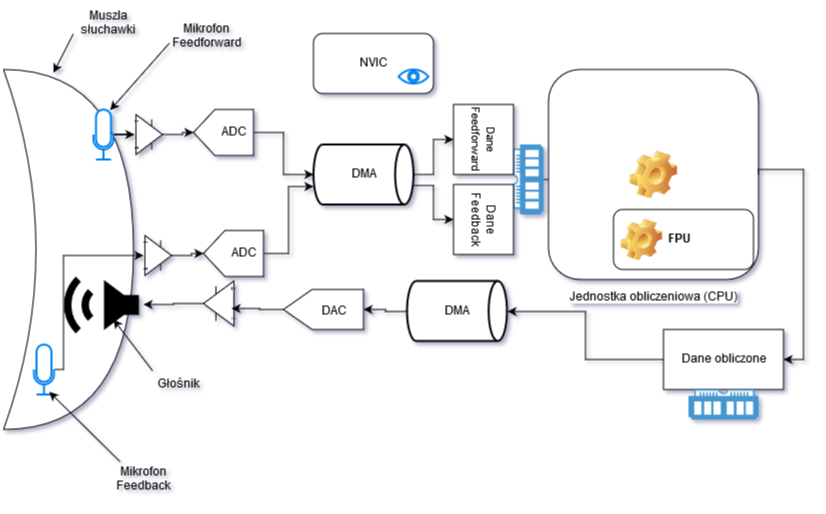
\includegraphics[width=\linewidth]{../Assets/schemat_ukladu.png}	
	\caption{Schemat układu.}
	\label{fig:schemat1}
\end{figure}
Autor pominął pomniejsze elementy, które nie wnoszą szczególnych informacji do modelu układu. W~kwestii umiejscowienia mikrofonu odsłuchowego autor posłużył się wnioskami wypracowanymi w~artykule dotyczącym aktywnej redukcji hałasu w~zastosowaniach słuchawek tłumiących \cite{ANC4HP}. Autorzy pracy na podstawie widma częstotliwościowego wyznaczyli optymalne położenie mikrofonu i~wykazali, że takim miejscem jest bliskie otoczenie przewodu słuchowego zewnętrznego. Konkretne położenie mikrofonu odsłuchowego ilustruje lokacja nr~8 na grafice \ref{fig:error_mic_placement} zapożyczonej z~wyżej wymienionej pracy. %TODO sprawdzic dopisek przy obrazku
Mikrofon odsłuchowy umiejscowiony w~optymalnej pozycji charakteryzuje się zlinearyzowaną odpowiedzią częstotliwościową, co ogranicza błędy pomiarowe i~poprawia precyzję zastosowanego rozwiązania. 
\begin{figure}
	\centering
	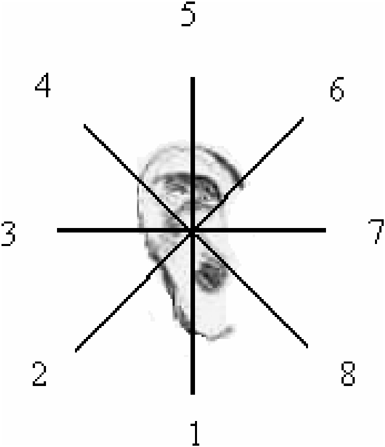
\includegraphics[scale=0.75]{../Assets/error_mic_placement.png}
	\caption{Położenie mikrofonu odsłuchowego odzwierciedla lokacja nr 8.}
	\label{fig:error_mic_placement}
\end{figure}
Aby stworzyć odgrodzoną przestrzeń sferyczną, autor postanowił złączyć (ścisnąć) dwie odłączone słuchawki użytych nauszników. Do celów testowych nie będzie potrzebny dodatkowy mikrofon umieszczony w~środku przestrzeni, zamiast tego zostanie użyty zamontowany już mikrofon odsłuchowy. Dane z~niego, oprócz do pamięci, zostaną wysłane również do komputera walidującego rozwiązanie, gdzie na bieżąco monitorowane będzie widmo częstotliwościowe.

Aby zasilić prototyp, autor podłączył mikrokontroler poprzez USB do komputera osobistego. Zapewniło to standardowe zasilanie na poziomie \SI{3.3}{\V}. Ponadto, celem odseparowania części analogowej od cyfrowej, autor zdecydował się zapewnić osobne zasilanie dla układów analogowych, a~więc mikrofonu wraz z~jego przedwzmacniaczem, oraz dla wzmacniacza głośnikowego. Tym samym zredukowane są zakłócenia, które normalnie mogłyby się przenieść z~linii zasilania układu cyfrowego do bardzo wrażliwej na te zakłócenia części analogowej. Zasilanie to zostało osiągnięte poprzez podpięcie pastylkowych akumulatorów \SI{3}{\V} do elementów analogowych. Zastosowanie ładowalnych akumulatorów zwiększa żywotność układu ograniczając liczbę potrzebnych wymian baterii.